\section{Metodología.}
\subsection{Definición del variables}
Teniendo en cuenta la explicación proporcionada en el apartado 2, podemos establecer que nuestro sistema contará con tres variables de salida: una para indicar la adecuación de atacar (a la que nos referiremos simplemente como \textit{Atacar} de ahora en adelante), una para indicar la adecuación de curarse (\textit{Curación}) y una última para la adecuación de defenderse (\textit{Defensa}).
Empecemos por plantear los factores que afectan a cada una de estas variables de manera más directa:
\begin{itemize}
	\item \textit{Atacar:} está condicionada por el daño que podemos causar a nuestro adversario, la vida con la que esperamos quedarnos si decidimos realizar esta acción y la probabilidad de acertar nuestro golpe o precisión.
	\item \textit{Defensa:} está condicionada, en principio, por la vida con la que esperaríamos quedarnos al realizar esta acción.
	\item \textit{Curación:} se encuentra en la misma situación que Defensa, depende de la vida con la que se quedaría el personaje si realizara esta acción.
\end{itemize}

Dadas estas consideraciones, podemos establecer las siguientes variables de entrada:

\begin{itemize}
	\item \textit{Vida restante después de atacar} (\textit{VRA}, para abreviar): Proporción de vida esperada del personaje controlado por el sistema de lógica difusa si éste decidiera atacar, con valores entre [0, 1]. Hay distintas formas en las que se podría calcular el valor de esta variable, y dependería del criterio de quien utilizara el sistema difuso. Por ejemplo, podría utilizarse la vida esperada en el peor, lo que conllevaría una estrategia más conservadora, pero también podría utilizarse una estimación del caso más probable, el mejor y el peor. En cualquier caso, el método elegido para calcular este valor no es competencia de nuestro sistema.
	\item \textit{DAÑO}: Proporción de vida perdida por el enemigo al recibir el ataque, entre [0, 1]. 
	\item \textit{Precisión (PREC)}: Probabilidad de que nuestro ataque acierte al enemigo, entre [0, 1].
	\item \textit{Vida restante después de defenderse (VRD):} Proporción de vida esperada del personaje controlado por el sistema de lógica difusa si éste decidiera defenderse, entre [0, 1]. Se le aplica lo mismo que a VRA.
	\item \textit{Vida restante después de curarse (VRC):} Proporción de vida esperada del personaje controlado por el sistema de lógica difusa si éste decidiera curarse, entre [0, 1]. Se le aplica lo mismo que a VRA. 
\end{itemize}

La razón de que estas variables sean estimaciones es porque en el cálculo de su valor de entrada pueden tenerse en cuenta diversos factores como considerar que el enemigo decida defenderse, o bien cuán probable sería hacer más daño del normal al atacar (lo que se conoce como golpe crítico).

Por otro lado, es conveniente poder determinar cuándo se espera que uno de los combatientes sobreviva y cuándo no. Por ello tenemos:

\begin{itemize}
	\item \textit{El enemigo sobrevive (ES):} Indica de manera categórica si el enemigo sobrevive al ataque teniendo en cuenta los datos proporcionados.
	\item\textit{El personaje sobrevive (PS):} Indica de manera categórica si el personaje controlado por el sistema sobrevive en caso de que decidiera atacar teniendo en cuenta los datos proporcionados.
\end{itemize}

\subsection{Precondiciones de las variables.}
Existen una serie de requisitos que deben cumplir las variables de entrada para garantizar que el sistema puede trabajar correctamente.
\begin{itemize}
	\item La Vida restante después de curarse (VRC) y la Vida restante después de defenderse (VRD) deben ser siempre mayores o iguales a la Vida restante después de atacar (VRA). Esto se debe a que, de otro modo, las acciones Defensa y Curación perderían sentido ya que se utilizan para perder menos vida, y se estaría perdiendo más.
	
	\item El DAÑO realizado al enemigo se entiende que siempre es mayor que cero, ya que en este tipo de juegos no se suele permitir un daño nulo.
	
	\item Si el Personaje Sobrevive (PS = sí), se entiende que la Vida restante después de atacar (VRA) tiene que ser mayor que cero. Y al contrario, si PS = no, VRA = 0.
	
\end{itemize}



\subsection{Representación gráfica de las variables.}
A continuación mostramos gráficamente cómo han quedado las variables de entrada y salida una vez difuminadas.
\subsubsection{Variables de entrada:}
\begin{figure}[H]
	\centering
	\begin{minipage}{.5\textwidth}
		\centering
		\includegraphics[scale=0.67]{images/variables/daño.png}
		\captionof{figure}{DAÑO}
	\end{minipage}%
	\begin{minipage}{.5\textwidth}
		\centering
		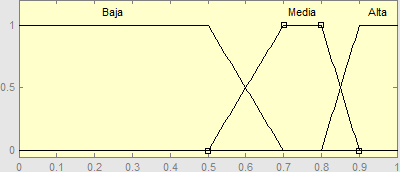
\includegraphics[scale=0.67]{images/variables/pa.png}
		\captionof{figure}{PREC}
	\end{minipage}
\end{figure}

\begin{figure}[H]
	\centering
	\begin{minipage}{.5\textwidth}
		\centering
		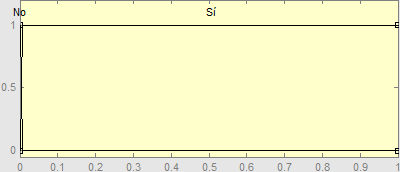
\includegraphics[scale=0.67]{images/variables/es.png}
		\captionof{figure}{ES}
	\end{minipage}%
	\begin{minipage}{.5\textwidth}
		\centering
		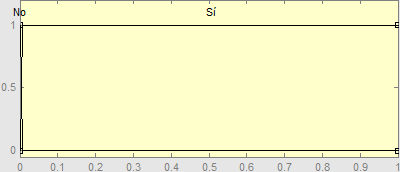
\includegraphics[scale=0.67]{images/variables/ps.png}
		\captionof{figure}{PS}
	\end{minipage}
\end{figure}

\begin{figure}[H]
	\centering
	\begin{minipage}{.5\textwidth}
		\centering
		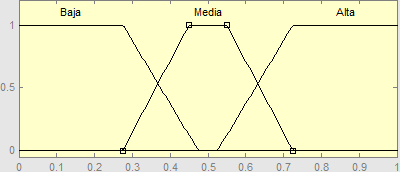
\includegraphics[scale=0.67]{images/variables/vrpa.png}
		\captionof{figure}{VRA}
	\end{minipage}%
	\begin{minipage}{.5\textwidth}
		\centering
		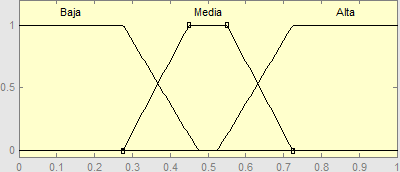
\includegraphics[scale=0.67]{images/variables/vrpc.png}
		\captionof{figure}{VRC}
	\end{minipage}
\end{figure}

\begin{figure}[H]
	\centering
	\begin{minipage}{.5\textwidth}
		\centering
		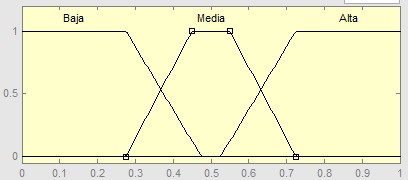
\includegraphics[scale=0.67]{images/variables/vrpd.png}
		\captionof{figure}{VRD}
	\end{minipage}%
	\begin{minipage}{.5\textwidth}
		\centering
	\end{minipage}
\end{figure}


\subsubsection{Variables de salida:}


\begin{figure}[H]
	\centering
	\begin{minipage}{.5\textwidth}
		\centering
		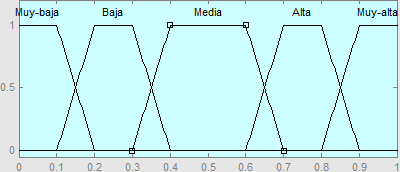
\includegraphics[scale=0.67]{images/variables/salida.png}
		\captionof{figure}{Ataque}
	\end{minipage}%
	\begin{minipage}{.5\textwidth}
		\centering
		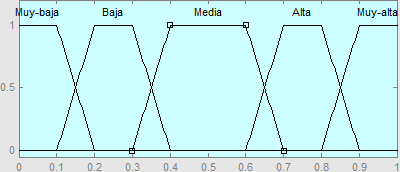
\includegraphics[scale=0.67]{images/variables/salida.png}
		\captionof{figure}{Defensa}
	\end{minipage}
\end{figure}

\begin{figure}[H]
	\centering
	\begin{minipage}{.5\textwidth}
		\centering
		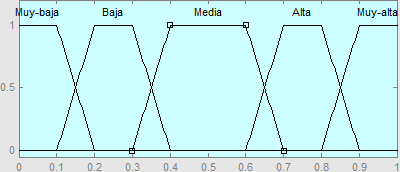
\includegraphics[scale=0.67]{images/variables/salida.png}
		\captionof{figure}{Curación}
	\end{minipage}
\end{figure}

\subsection{Definición de criterios y reglas.}
Para la creación de las reglas hemos optado por una estrategia ofensiva en la que se tiende a priorizar el ataque sobre las otras acciones, que van adquiriendo relevancia cuando la situación se vuelve desfavorable para el personaje (vida baja, el personaje no sobrevive al próximo ataque enemigo…). En estos casos, la adecuación del ataque va bajando en favor de la curación y la defensa. Para discernir entre estas dos últimas, nos basamos en cuál de ellas nos va a dejar en una situación más ventajosa, es decir, cuál nos permitirá terminar el turno con más vida.

Llegados a este punto, el lector podría estar preguntándose qué sucede si, por ejemplo, el próximo ataque enemigo podría dejar al personaje con baja vida, pero en el momento de hacer los cálculos la vida del personaje es alta. ¿Daría esto prioridad a la curación cuando en verdad sería una curación ``desperdiciada'' porque la vida ya era alta? No necesariamente. Teniendo en cuenta que nuestra acción va antes que la del adversario y que siempre se considera la vida esperada para cada acción al final del turno, una curación en estas condiciones resultaría en una vida restante tras curarse igual o muy similar a la de atacar, lo que impediría que cobrase una relevancia que no le corresponde.

El mismo tipo de razonamiento puede ser aplicado a casos similares, y ha sido la forma de pensar en el momento de elaborar las reglas.

\noindent\texttt{1. If PREC is Alta and ES is No then Curación is Muy-baja, Defensa is Muy-baja, Ataque is Muy-alta\\\newline
2. If PREC is Media and ES is No then Curación is Baja, Defensa is Baja, Ataque is Muy-alta\\\newline
3. If VRC is Alta and VRD is Media and PS is No then Curación is Muy-alta, Defensa is Alta, Ataque is Muy-baja\\\newline
4. If VRC is Alta and VRD is Baja and PS is No then Curación is Muy-alta, Defensa is Media, Ataque is Muy-baja\\\newline
5. If VRC is Media and VRD is Baja and PS is No then Curación is Alta, Defensa is Media, Ataque is Muy-baja\\\newline
6. If VRC is Baja and VRD is Media and PS is No then Curación is Media, Defensa is Alta, Ataque is Muy-baja\\\newline
7. If VRC is Baja and VRD is Alta and PS is No then Curación is Media, Defensa is Muy-alta, Ataque is Muy-baja\\\newline
8. If VRC is Media and VRD is Alta and PS is No then Curación is Alta, Defensa is Muy-alta, Ataque is Muy-baja\\\newline
9. If VRC is Baja and VRD is Baja and PS is No then Curación is Media, Defensa is Media, Ataque is Muy-baja\\\newline
10. If VRC is Media and VRD is Media and PS is No then Curación is Alta, Defensa is Alta, Ataque is Muy-baja\\\newline
11. If VRC is Alta and VRD is Alta and PS is No then Curación is Muy-alta, Defensa is Muy-alta, Ataque is Muy-baja\\\newline
12. If PREC is Alta and DAÑO is Alto and ES is Sí and PS is Sí then Curación is Muy-baja, Defensa is Muy-baja, Ataque is Muy-alta\\\newline
13. If PREC is Media and DAÑO is Alto and ES is Sí and PS is Sí then Curación is Muy-baja, Defensa is Muy-baja, Ataque is Muy-alta\\\newline
14. If PREC is Media and DAÑO is Medio and ES is Sí and PS is Sí then Curación is Muy-baja, Defensa is Muy-baja, Ataque is Muy-alta\\\newline
15. If PREC is Alta and DAÑO is Medio and ES is Sí and PS is Sí then Curación is Muy-baja, Defensa is Muy-baja, Ataque is Muy-alta\\\newline
16. If PREC is Alta and VRA is Alta and DAÑO is Bajo and ES is Sí and PS is Sí then Curación is Muy-baja, Defensa is Muy-baja, Ataque is Alta\\\newline
17. If PREC is Media and VRA is Alta and DAÑO is Bajo and ES is Sí and PS is Sí then Curación is Muy-baja, Defensa is Muy-baja, Ataque is Alta\\\newline
18. If PREC is Alta and VRA is Media and DAÑO is Bajo and ES is Sí and PS is Sí then Curación is Baja, Defensa is Baja, Ataque is Alta\\\newline
19. If PREC is Media and VRA is Media and DAÑO is Bajo and ES is Sí and PS is Sí then Curación is Baja, Defensa is Baja, Ataque is Media\\\newline
20. If PREC is Baja and VRA is Alta and ES is Sí and PS is Sí then Curación is Baja, Defensa is Baja, Ataque is Media\\\newline
21. If PREC is Baja and VRA is Media and ES is Sí and PS is Sí then Curación is Baja, Defensa is Baja, Ataque is Media\\\newline
22. If VRC is Baja and VRD is Baja and VRA is Baja and ES is Sí and PS is Sí then Curación is Baja, Defensa is Baja, Ataque is Media\\\newline
23. If VRC is Media and VRD is Baja and VRA is Baja and ES is Sí and PS is Sí then Curación is Media, Defensa is Baja, Ataque is Baja\\\newline
24. If VRC is Alta and VRD is Baja and VRA is Baja and ES is Sí and PS is Sí then Curación is Alta, Defensa is Baja, Ataque is Baja\\\newline
25. If VRC is Baja and VRD is Media and VRA is Baja and ES is Sí and PS is Sí then Curación is Baja, Defensa is Media, Ataque is Baja\\\newline
26. If VRC is Media and VRD is Media and VRA is Baja and ES is Sí and PS is Sí then Curación is Media, Defensa is Media, Ataque is Baja\\\newline
27. If VRC is Alta and VRD is Media and VRA is Baja and ES is Sí and PS is Sí then Curación is Alta, Defensa is Media, Ataque is Baja\\\newline
28. If VRC is Baja and VRD is Alta and VRA is Baja and ES is Sí and PS is Sí then Curación is Baja, Defensa is Alta, Ataque is Baja\\\newline
29. If VRC is Media and VRD is Alta and VRA is Baja and ES is Sí and PS is Sí then Curación is Media, Defensa is Alta, Ataque is Baja\\\newline
30. If VRC is Alta and VRD is Alta and VRA is Baja and ES is Sí and PS is Sí then Curación is Alta, Defensa is Alta, Ataque is \\\newline
31. If VRC is Baja and PREC is Baja and VRD is Baja and ES is No and PS is Sí then Curación is Baja, Defensa is Baja, Ataque is Media\\\newline
32. If VRC is Media and PREC is Baja and VRD is Baja and ES is No and PS is Sí then Curación is Media, Defensa is Baja, Ataque is Baja\\\newline
33. If VRC is Alta and PREC is Baja and VRD is Baja and ES is No and PS is Sí then Curación is Alta, Defensa is Baja, Ataque is Baja\\\newline
34. If VRC is Baja and PREC is Baja and VRD is Media and ES is No and PS is Sí then Curación is Baja, Defensa is Media, Ataque is Baja\\\newline
35. If VRC is Media and PREC is Baja and VRD is Media and ES is No and PS is Sí then Curación is Media, Defensa is Media, Ataque is Baja\\\newline
36. If VRC is Alta and PREC is Baja and VRD is Media and ES is No and PS is Sí then Curación is Alta, Defensa is Media, Ataque is Baja\\\newline
37. If VRC is Baja and PREC is Baja and VRD is Alta and ES is No and PS is Sí then Curación is Baja, Defensa is Alta, Ataque is Baja\\\newline
38. If VRC is Media and PREC is Baja and VRD is Alta and ES is No and PS is Sí then Curación is Media, Defensa is Alta, Ataque is Baja\\\newline
39. If VRC is Alta and PREC is Baja and VRD is Alta and ES is No and PS is Sí then Curación is Alta, Defensa is Alta, Ataque is Baja
}